\documentclass{gtpart}
\usepackage{amsmath,amssymb,amsthm,stmaryrd}
\usepackage[all]{xy}
\usepackage{tikz}
\usepackage{url}
\usepackage{hyperref}
\usepackage{enumerate}
\usepackage{tensor}
%/home/grad/zyf/TeX/inputs/
\usepackage{mathrsfs}
\usepackage{graphicx}
\usepackage{mathtools}
%\usepackage{amsrefs}
%\usepackage{setspace}
%\doublespacing

\title{The power operation structure on Morava $E$-theory of height 2 at the prime 3}
\author{Yifei Zhu}
\givenname{Yifei}
\surname{Zhu}
\address{Department of Mathematics\\University of Minnesota\\Minneapolis, MN 55455\\USA}
\email{zyf@math.umn.edu}

%\subject{primary}{msc2000}{55P99}
%\subject{secondary}{msc2000}{55Q99}

%\bibliographystyle{gtart}
\parskip 0.7pc
\parindent 0pt

\newtheorem{thm}{Theorem}
\newtheorem{cor}[thm]{Corollary}
\newtheorem{prop}[thm]{Proposition}
\newtheorem{lem}[thm]{Lemma}
\theoremstyle{definition}
\newtheorem{defn}[thm]{Definition}
\theoremstyle{remark}
\newtheorem{rmk}[thm]{Remark}
\newtheorem{ex}[thm]{Example}
\newtheorem{case}[thm]{Case}
\newtheorem{slogan}[thm]{Slogan}
\newtheorem{ques}[thm]{Question}

\def\co{\colon\thinspace}
\newcommand{\mb}[1]{\mathbb{#1}}
\newcommand{\mf}[1]{\mathfrak{#1}}

\newcommand{\NB}[1]{{\bf (NB: #1)}}

\newcommand{\Ext}{\ensuremath{{\rm Ext}}}
\newcommand{\Coext}{\ensuremath{{\rm Coext}}}
\newcommand{\Hom}{\ensuremath{{\rm Hom}}}
\newcommand{\Tor}{\ensuremath{{\rm Tor}}}
\newcommand{\Ind}{\ensuremath{{\rm Ind}}}
\newcommand{\Res}{\ensuremath{{\rm Res}}}
\newcommand{\colim}{\ensuremath{\mathop{\rm colim}}}
\newcommand{\hocolim}{\ensuremath{\mathop{\rm hocolim}}}
\newcommand{\holim}{\ensuremath{\mathop{\rm holim}}}
\newcommand{\overto}{\mathop\rightarrow}
\newcommand{\overfrom}{\mathop\leftarrow}
\newcommand{\into}{\mathop\hookrightarrow}
\newcommand{\onto}{\mathop\twoheadrightarrow}
\newcommand{\longoverto}{\mathop{\longrightarrow}}
\newcommand{\Irr}{\ensuremath{\mathop{\rm Irr}}}
\newcommand{\Rep}{\ensuremath{\mathop{\rm Rep}}}
\newcommand{\Map}{\ensuremath{{\rm Map}}}
\newcommand{\GL}{{\rm GL}}
\newcommand{\Uni}{{\rm U}}
\newcommand{\BU}{{\rm BU}}
\newcommand{\Sp}{{\cal S}p}
\newcommand{\Sym}{{\rm Sym}}
\newcommand{\thh}{{\rm thh}}
\newcommand{\TAF}{{\rm TAF}}
\newcommand{\TAQ}{{\rm TAQ}}
\newcommand{\End}{{\rm End}}
\newcommand{\Aut}{{\rm Aut}}
\newcommand{\As}{{\cal A}s}
\newcommand{\LT}{{\rm LT}}
\newcommand{\Spec}{{\rm Spec\thinspace}}
\newcommand{\Proj}{{\rm Proj\thinspace}}
\newcommand{\Spf}{{\rm Spf}}
\newcommand{\tmf}{{\rm tmf}}
\newcommand{\eo}{{\rm eo}}
\newcommand{\TMF}{{\rm TMF}}
\newcommand{\Ell}{{\cal E}ll}
\newcommand{\Lie}{{\rm Lie}}
\newcommand{\Sh}{{\rm Sh}}
\newcommand{\HF}{{\rm H}{\mb F}}
\newcommand{\cF}{\overline {\mb F}}
\newcommand{\cQ}{\overline {\mb Q}}

\newcommand{\eilm}[1]{\ensuremath{{\mb H} #1}}
\newcommand{\smsh}[1]{\ensuremath{\mathop{\wedge}_{#1}}}
\newcommand{\tens}[1]{\ensuremath{\mathop{\otimes}_{#1}}}
\newcommand{\susp}{\ensuremath{\Sigma}}
\newcommand{\mapset}[3]{\ensuremath{\left[#2,#3\right]_{#1}}}
\newcommand{\form}[2]{\ensuremath{\left\langle#1,#2\right\rangle}}
\newcommand{\bilin}[2]{\ensuremath{\left(#1,#2\right)}}
\newcommand{\comp}[1]{\ensuremath{#1^\wedge}}
\newcommand{\loca}[3]{\ensuremath{L^{#1}_{#2}(#3)}}
\newcommand{\tc}[3]{\ensuremath{\Omega_{#2 / #1}^{#3}}}
\newcommand{\atc}[3]{\ensuremath{\L_{#2 / #1}^{#3}}}

\newcommand{\xym}[1]{
\vskip 0.7pc
\centerline{\xymatrix{#1}}
\vskip 0.7pc
}

\newcommand{\CA}{{\cal A}}
\newcommand{\Mod}{{\rm Mod}}
\newcommand{\Alg}{{\rm Alg}}
\newcommand{\Frob}{{\rm Frob}}
\newcommand{\DF}{{{\rm DefFrob}_\Gamma}}
\newcommand{\Model}{{\rm Model}}
\newcommand{\Gm}{{{\mb G}_m}}
\newcommand*{\longhookrightarrow}{\ensuremath{\lhook\joinrel\relbar\joinrel\rightarrow}}
\newcommand{\cf}{cf.\thinspace}

\newcommand{\DL}{Dyer-Lashof~}
\newcommand{\BF}{{\mb F}}
\newcommand{\BG}{{\mb G}}
\newcommand{\BP}{{\mb P}}
\newcommand{\BZ}{{\mb Z}}
\newcommand{\HC}{\widehat{C}}
\newcommand{\HS}{\widehat{S}}
\newcommand{\Tf}{\widetilde{f}}
\newcommand{\Tp}{\widetilde{\psi}}
\newcommand{\md}{~~{\rm mod}~}
\newcommand{\ad}{{\rm and}}
\newcommand{\A}{\alpha}
\newcommand{\G}{\Gamma}
\newcommand{\g}{\gamma}
\newcommand{\K}{\kappa}
\newcommand{\p}{\psi^3}
\newcommand{\s}{S^\bullet}
\newcommand{\isog}[1]{Proposition \ref{prop:isog}\thinspace \eqref{isog(#1)}}
\newcommand{\q}[1]{Proposition \ref{prop:Q}\thinspace \eqref{Q(#1)}}
\newcommand{\go}[1]{Definition \ref{def:go}\thinspace \eqref{go(#1)}}


%single word
%end space
%page break
%labels
%newcommands
%.bib
%line break .tex


\begin{document}
\begin{abstract}
 We give explicit calculations of the algebraic theory of power operations for a specific Morava $E$-theory spectrum and its $K(1)$-localization.  
 These power operations arise from the universal degree-3 isogeny of elliptic curves associated to the $E$-theory.  
\end{abstract}


\maketitle
\section{Introduction}

Suppose $E$ is a commutative $S$-algebra, in the sense of \cite{EKMM}, and $A$ is a commutative $E$-algebra.  
We want to capture the properties and underlying structure of the homotopy groups $\pi_* A = A_*$ of $A$, 
by studying operations associated to the cohomology theory that $E$ represents.  

An important family of cohomology operations, called {\em power operations}, is constructed via the extended powers.  
Specifically, consider the {\em $m$'th extended power} functor 
\[
 \BP_E^m (-) \coloneqq (-)^{\wedge_E m} / \Sigma_m \co \Mod_E \to \Mod_E 
\]
on the category of $E$-modules which sends an $E$-module to its $m$-fold smash product over $E$ modulo the action by the symmetric group on $m$ letters.  
The $\BP_E^m (-)$'s assemble together to give the {\em free commutative $E$-algebra} functor 
\[
 \BP_E (-) \coloneqq \bigvee_{m \geq 0} \BP_E^m (-) \co \Mod_E \to \Alg_E 
\]
from the category of $E$-modules to the category of commutative $E$-algebras.  
These functors descend to homotopy categories.  
In particular, each $\A \in \pi_{d+i}~\BP_E^m (\Sigma^d E)$ gives rise to a power operation 
\[
 Q_\A \co A_d \to A_{d+i} 
\]
(\cf \cite[Sections I.2 and IX.1]{H_infty} and \cite[Section 3]{cong}).  

Under the action of power operations, $A_*$ is an algebra over some operad in $E_*$-modules involving the structure of $E_* B\Sigma_m$ for all $m$.  
This operad is traditionally called a {\em \DL algebra}, or more precisely, 
a \DL {\em theory} as the {\em algebraic theory} of power operations acting on the homotopy groups of commutative $E$-algebras 
(\cf \cite[Chapters III, VIII, and IX]{H_infty} and \cite[Section 9]{lpo}).  

A specific case is when $E$ represents a Morava $E$-theory of height $n$ and $A$ is $K(n)$-local.  
Morava $E$-theory spectra are of crucial importance in modern stable homotopy theory, 
particularly in the work of Ando, Hopkins, and Strickland \cite{cube}.  
Much of the $K(n)$-local $E$-\DL theory has been worked out by those authors (\cf \cite[1.5]{cong} for a description of the history).  
In \cite{cong} Rezk gives a unified treatment of this \DL theory.  
He works out a congruence criterion that must hold in an algebra over the \DL theory (\cite[Theorem A]{cong}).  
This enables one to study the \DL {\em theory}, which models all the algebraic structure naturally adhering to $A_*$, 
by working with a certain associative ring $\G$ as the \DL {\em algebra}.  
Moreover, Rezk provides a geometric description of this congruence criterion, 
in terms of sheaves on the moduli problem of deformations of formal groups and Frobenius isogenies (\cf \cite[Theorem B]{cong}).  
This connects the structure of $\G$ to the geometry underlying $E$, 
moving one step forward from a workable object $\G$ to things that are computable.  
Based on these, in a companion paper \cite{h2p2}, 
Rezk gives explicit calculations of the \DL theory for a specific Morava $E$-theory of height $n = 2$ at the prime 2.  

The purpose of this paper is to make available calculations analogous to some of the results in \cite{h2p2}, at the prime 3, 
together with calculations of the corresponding power operations on the $K(1)$-localization of the Morava $E$-theory spectrum.  


\subsection{Outline of the paper}

As in \cite{h2p2}, the computation of power operations in this paper follows the approach of \cite{steenrod}: 
One first defines a total power operation, 
and then uses the computation of the cohomology of the classifying space $B\Sigma_m$ for the symmetric group to obtain individual power operations.  
These two steps are carried out in Sections \ref{sec:total} and \ref{sec:individual} respectively.  

In Section \ref{sec:total}, by doing calculations with elliptic curves associated to our Morava $E$-theory $E$, 
we give formulas for the total power operation $\p$ on $E_0$ and the ring $S_3$ which represents the corresponding moduli problem.  

In Section \ref{sec:individual}, based on calculations of $E^* B\Sigma_m$ in \cite{Str98} as reflected in the formula for $S_3$, 
we define individual power operations, and derive the relations they satisfy.  
In view of the general structures studied in \cite{cong}, 
we then get an explicit description of the \DL algebra $\G$ for $K(2)$-local commutative $E$-algebras.  

In Section \ref{sec:K(1)}, we describe the relationship between the total power operation $\p$, at height 2, and the corresponding $K(1)$-local power operations.  
We then derive formulas for the latter from the calculations in Section \ref{sec:total}.  

\begin{rmk}
\label{rmk:grading}
 In Section \ref{sec:total}, we do calculations with a universal elliptic curve 
 over {\em all} of the moduli stack which is an affine open subscheme 
 of a weighted projective space (\cf Proposition \ref{prop:C}).  
 At the prime 3, the supersingular locus consists of a single closed point, 
 and the corresponding Morava $E$-theory arises {\em locally} 
 in an affine coordinate chart of this weighted projective space containing the supersingular locus.  
 In this paper we choose a particular affine coordinate chart 
 for computing the homotopy groups of the $E$-theory spectrum and the power operations; 
 we hope that the generality of the calculations in Section \ref{sec:total} 
 makes it easier to work with other coordinate charts as well.  
\end{rmk}

\begin{rmk}
\label{rmk:parameter}
 The ring $S_3$ turns out to be an algebra with one generator over the base ring where our elliptic curve is defined 
 (\cf \isog{i} and \eqref{S_3}).  This generator appears as a parameter in the formulas for the total power operation $\p$, 
 and is responsible for how the individual power operations are defined and how their formulas look.  
 Different choices of this parameter result in different bases of the \DL algebra $\G$.  
 The parameter in this paper comes from the relative cotangent space of the elliptic curve at the identity 
 (\cf \isog{iv}, Corollary \ref{cor:K'}, and Remark \ref{rmk:K'}).  
 This choice is convenient for deriving Adem relations in \q{iv}, 
 and it fits into the treatment of gradings in \cite[Section 2]{cong} (\cf \go{ii} and Theorem \ref{thm:gamma}).  
 We should point out that our choice is by no means canonical.  
 We do not know yet, as part of the structure of the \DL algebra, 
 if there is a canonical basis which is both geometrically interesting and computationally convenient.  
 Somewhat surprisingly, although it appears to come from different considerations, 
 our choice has an analog at the prime 2 which coincides with the parameter used in \cite{h2p2} (\cf Remarks \ref{rmk:K} and \ref{rmk:KK'}).  
 The calculations follow a recipe in hope of generalizing to other Morava $E$-theories of height 2; 
 we hope to address these matters and recognize more of the general patterns based on further computational evidence.  
\end{rmk}


\subsection{Acknowledgements}

I thank Charles Rezk for his encouragement on this work, and for his observation in a correspondence which led to Proposition \ref{prop:frob^2} and Corollary \ref{cor:K'}.  

I thank Kyle Ormsby for helpful discussions on Section \ref{sec:total}, and for directing me to places in the literature.  

I thank Tyler Lawson for the sustained support from him I received as a student.  


\subsection{Conventions}

Let $p$ be a prime, $q$ a power of $p$, and $n$ a positive integer.  We use the symbols 
\[
 \BF_q\text{,}~~\BZ_q\text{,}~~\ad~~\BZ/n 
\]
to denote a field with $q$ elements, the ring of $p$-typical Witt vectors over $\BF_q$, 
and the additive group of integers modulo $n$, respectively.  

If $R$ is a ring, then $R\llbracket x \rrbracket$ and $R (\!(x)\!)$ denote the rings of formal power series and formal Laurent series over $R$ in the variable $x$ respectively.  
If $I \subset R$ is an ideal, then $R_I^\wedge$ denotes the completion of $R$ with respect to $I$.  

If $E$ is an elliptic curve and $m$ is an integer, then $[m]$ denotes the multiplication-by-$m$ map on $E$, and $E[m]$ denotes the $m$-torsion subgroup of $E$.  

All formal groups mentioned in this paper will be commutative and one-dimensional.  

The terminology for the structure of the \DL theory will follow \cite{cong} and \cite{h2p2}; 
some of the notions there are taken in turn from \cite{BW} and \cite{V}.  


\section{Total power operations}
\label{sec:total}

\subsection{A universal elliptic curve and a Morava $E$-theory spectrum}
\label{subsec:ec}

A Morava $E$-theory of height 2 at the prime 3 has its formal group as 
the universal deformation of a height-2 formal group over a perfect field of characteristic 3.  
Given a supersingular elliptic curve over such a field, 
its formal completion at the identity produces a formal group of height 2.  
To study power operations for the corresponding Morava $E$-theory, 
we do calculations with the universal deformation of that supersingular elliptic curve 
which is a family of elliptic curves with a $\G_1(N)$-structure (\cf \cite[Section 3.2]{KM}) where $N$ is prime to 3.  
Here is a specific model (\cf \cite[4(4.6a)]{ec}).  

\begin{prop}
\label{prop:C}
 Over $\BZ [1/4]$, the moduli problem of nonsingular elliptic curves with a choice of 
 a point of exact order 4 and a nowhere-vanishing invariant one-form is represented by 
 \begin{equation}
 \label{Cxy}
  C \co y^2 + a x y + a b y = x^3 + b x^2 
 \end{equation}
 with chosen point $(0,0)$ and one-form $dx / (2 y + a x + a b) = dy / (3 x^2 + 2 b x - a y)$ 
 over the graded ring 
 \[
  \s \coloneqq \BZ [1/4] [a, b, \Delta^{-1}] 
 \]
 where $|a| = 1$, $|b| = 2$, and $\Delta = a^2 b^4 (a^2 - 16 b)$.  
\end{prop}
\begin{proof}
 Let $P$ be the chosen point of exact order 4.  
 Since $2P$ is 2-torsion, the tangent line of the elliptic curve at $P$ passes through $2P$, 
 and the tangent line at $2P$ passes through the identity at the infinity.  
 With this observation, the rest of the proof is analogous to that of \cite[Proposition 3.2]{tmf3}.  
\end{proof}

Over a finite field of characteristic 3, $C$ is supersingular precisely when the quantity 
\begin{equation}
\label{H}
 H \coloneqq a^2 + b 
\end{equation}
vanishes (\cf \cite[V.4.1a]{AEC}).  
As $(3,H)$ is a maximal ideal of $\s$ corresponding to the closed subscheme $\Spec \BF_3$, 
the supersingular locus consists of a single closed point, 
and $C$ restricts to $\BF_3$ as 
\[
 C_0 \co y^2 + x y - y = x^3 - x^2.  
\]

From the above universal deformation $C$ of $C_0$, we next produce a Morava $E$-theory spectrum which is 2-periodic.  
We follow the convention that elements in algebraic degree $n$ lie in topological degree $2n$, and work in an affine \'etale coordinate chart of 
the weighted projective space $\Proj \BZ [1/4] [a, b]$ (\cf Remark \ref{rmk:grading}).  
Define elements $u$ and $c$ such that 
\[
 a = u c \qquad \ad \qquad b = u^2.  
\]
Consider the graded ring 
\[
 \s [u^{-1}] \cong \BZ [1/4] [a, \Delta^{-1}] [u^{\pm1}] 
\]
where $|u| = 1$, and denote by $S$ its subring of elements in degree 0 so that 
\begin{equation}
\label{S}
 S \cong \BZ [1/4] [c, \delta^{-1}] 
\end{equation}
where $\delta = u^{-12} \Delta = c^2 (c^2 - 16)$.  Write 
\[
 \HS = \BZ_9 \llbracket h \rrbracket 
\]
where 
\begin{equation}
\label{h}
 h \coloneqq u^{-2} H = c^2 + 1.  
\end{equation}
Let $i$ be an element generating $\BZ_9$ over $\BZ_3$ with $i^2 = -1$.  
We may choose 
\[
 c \equiv i \md (3,h) 
\]
and we have 
\[
 \delta \equiv -1 \md (3,h) 
\]
where $(3,h)$ is the maximal ideal of the complete local ring $\HS$.  
Then by Hensel's lemma, both $c$ and $\delta$ lie in $\HS$, and both are invertible.  Thus 
\[
 \HS \cong S_{(3,h)}^\wedge.  
\]

Now $C$ restricts to $S$ as 
\begin{equation}
\label{Cc}
 y^2 + c x y + c y = x^3 + x^2.  
\end{equation}
Let $\HC$ be the formal completion of $C$ over $S$ at the identity.  
It is a formal group over $\HS$, and its reduction to $\BF_9 = \HS / (3,h)$ 
is a formal group $\BG$ of height 2 in view of \eqref{h} and \eqref{H}.  
By the Serre-Tate theorem (\cf \cite[2.9.1]{KM}), 
3-adically the deformation theory of an elliptic curve is equivalent to 
the deformation theory of its 3-divisible group, 
and thus $\HC$ is the universal deformation of $\BG$ in view of Proposition \ref{prop:C}.  
Let $E$ be the $E_\infty$-ring spectrum which represents the Morava $E$-theory 
associated to $\BG$ (\cf \cite[Corollary 7.6]{GH}).  Then 
\[
 E_* \cong \BZ_9 \llbracket h \rrbracket [u^{\pm 1}] 
\]
where $u$ is in topological degree 2, and it corresponds to a local uniformizer at the identity of $C$.  


\subsection{Points of exact order 3}

To study $C$ in a formal neighborhood of the identity, it is convenient to make a change of variables.  
Let 
\[
 u = \frac{x}{y} \quad \ad \quad v = \frac{1}{y}, \qquad {\rm so} \qquad x = \frac{u}{v} \quad \ad \quad y = \frac{1}{v}.  
\]
The identity of $C$ is then $(u,v) = (0,0)$, with $u$ a local uniformizer.  
The equation \eqref{Cxy} of $C$ becomes 
\begin{equation}
\label{Cuv}
 v + a u v + a b v^2 = u^3 + b u^2 v.  
\end{equation}

\begin{prop}
\label{prop:tors}
 On the elliptic curve $C$ over $\s$, the $uv$-coordinates $(d,e)$ of any nonzero 3-torsion point satisfy the identities 
 \begin{equation}
 \label{f}
  f(d) = 0 
 \end{equation}
 and 
 \begin{equation}
 \label{g}
  e = g(d) 
 \end{equation}
 where $f, g \in \s [u]$ are given by 
 \begin{equation*}
 \begin{split}
  f(u) = & ~ b^4 u^8 + 3 a b^3 u^7 + 3 a^2 b^2 u^6 + (a^3 b + 7 a b^2) u^5 + (6 a^2 b - 6 b^2) u^4 + 9 a b u^3 \\
         & + (-a^2 + 8 b) u^2 - 3 a u - 3, \\
  g(u) = & -\frac{1}{a (a^2 - 16 b)} \big( a b^3 u^7 + (3 a^2 b^2 - 2 b^3) u^6 + (3 a^3 b -6 a b^2) u^5 + (a^4 + a^2 b \\
         & + 2 b^2) u^4 + (4 a^3 - 15 a b) u^3 + 18 b u^2 - 12 a u - 18 \big).  
 \end{split}
 \end{equation*}
\end{prop}
\begin{proof}
 \footnote{See Appendix \ref{apx:tors} for formulas for the polynomials $\Tf$, $Q_1$, $R_1$, $Q_2$, $R_2$, $K$, $L$, $M$, and $N$ that appear in the proof.  }
 Given the elliptic curve $C$ with equation \eqref{Cxy}, a nonzero point $Q$ is 3-torsion if and only if the polynomial 
 \[
  \psi_3 (x) \coloneqq 3 x^4 + (a^2 + 4 b) x^3 + 3 a^2 b x^2 + 3 a^2 b^2 x + a^2 b^3 
 \]
 vanishes at $Q$ (\cf \cite[Exercise 3.7f]{AEC}).  Substituting $x = u / v$ and clearing the denominators, we get a homogeneous polynomial 
 \[
  \Tp_3(u,v) \coloneqq 3 u^4 + (a^2 + 4 b) u^3 v + 3 a^2 b u^2 v^2 + 3 a^2 b^2 u v^3 + a^2 b^3 v^4.  
 \]
 As $Q = (d,e)$ in $uv$-coordinates, we then have 
 \begin{equation}
 \label{Tp}
  \Tp_3(d,e) = 0.  
 \end{equation}

 To get the polynomial $f$, we take $v$ as variable and rewrite \eqref{Cuv} as a quadratic equation 
 \begin{equation}
 \label{quadratic}
  a b v^2 + (-b u^2 + a u + 1) v - u^3 = 0 
 \end{equation}
 where the leading coefficient $a b$ is invertible in $\s = \BZ [1/4] [a, b, \Delta^{-1}]$ as $\Delta = a^2 b^4 (a^2 - 16 b)$.  
 Define 
 \begin{equation}
 \label{Tfdef}
  \Tf(u) \coloneqq \Tp_3(u,v) \Tp_3(u,\bar{v}) 
 \end{equation}
 where $v$ and $\bar{v}$ are formally the conjugate roots of \eqref{quadratic} 
 so that we compute $\Tf$ in terms of $u$ by substituting 
 \[
  v + \bar{v} = \frac{b u^2 - a u - 1}{a b} \qquad \ad \qquad v \bar{v} = -\frac{u^3}{a b}.  
 \]
 We then factor $\Tf$ over $\s$ as 
 \begin{equation}
 \label{Tffactor}
  \Tf(u) = -\frac{u^4 f(u)}{a^2 b} 
 \end{equation}
 with $f$ the stated degree-8 polynomial.  
 We check that $f$ is irreducible by applying Eisenstein's criterion to the maximal ideal $(3,H)$ of $\s$.  

 We have $\Tf(d) = 0$ by \eqref{Tfdef} and \eqref{Tp}.  
 To see $f(d) = 0$, consider the affine closed subscheme $D \subset C[3]$ of points of exact order 3.  
 By \cite[2.3.1]{KM} it is finite locally free of rank 8 over $\s$.  
 By the Cayley-Hamilton theorem, as a global section of $D$, $u$ locally satisfies a monic degree-8 equation, 
 and this equation locally defines the rank-8 scheme $D$.  
 Since $D$ is affine, it is then globally defined by a monic degree-8 equation in $u$.  
 We determine this equation in view of $\Tf(d) = 0$ and \eqref{Tffactor}, and (up to a unit in $\s$) get the first stated identity \eqref{f}.  

 To get the polynomial $g$, we note that both the quartic polynomial 
 \[
  A(v) \coloneqq \Tp_3(d,v) 
 \]
 and the quadratic polynomial 
 \[
  B(v) \coloneqq a b v^2 + (-b d^2 + a d + 1) v - d^3 
 \]
 vanish at $e$, and thus so does their greatest common divisor (gcd).  
 Applying the Euclidean algorithm (\cf Appendix \ref{apx:tors} for explicit expressions), we have 
 \begin{equation*}
 \begin{split}
  A(v) = & ~ Q_1(v) B(v) + R_1(v), \\
  B(v) = & ~ Q_2(v) R_1(v) + R_2, 
 \end{split}
 \end{equation*}
 where 
 \[
  R_1(v) = K(d) v + L(d) 
 \]
 for some polynomials $K$ and $L$, and $R_2 = 0$ in view of \eqref{f}.  Thus $R_1(v)$ is the gcd of $A(v)$ and $B(v)$, and hence 
 \[
  K(d) e + L(d) = R_1(e) = 0.  
 \]
 To write $e$ in terms of $d$ from the above identity, we apply the Euclidean algorithm to $f$ and $K$.  
 Their gcd turns out to be 1, and thus there are polynomials $M$ and $N$ with 
 \[
  M(u) f(u) + N(u) K(u) = 1.  
 \]
 By \eqref{f} we then have $N(d) K(d) = 1$, and thus 
 \[
  e = -N(d) L(d) = g(d) 
 \]
 where $g$ is as stated.  
\end{proof}

\begin{rmk}
\label{rmk:dmod3}
 The formula for $f$ in Proposition \ref{prop:tors} satisfies a congruence 
 \[
  f(u) \equiv u^2 (b^4 u^6 + a b H u^3 - H) \md 3.  
 \]
 The two roots (counted with multiplicity) of $f(u)$ which reduce to zero modulo 3 correspond to 
 the two nonzero points in the unique order-3 subgroup of $C$ in a formal neighborhood of the identity.  
\end{rmk}


\subsection{A universal isogeny and a total power operation}

\begin{prop}
\label{prop:isog}
 \mbox{}
 \begin{enumerate}[(i)]
  \item \label{isog(i)} The universal degree-3 isogeny $\psi$ with source $C$ is defined over the graded ring 
  \[
   \s_3 \coloneqq \s [\K] \big/ \big( W(\K) \big) 
  \]
  where $|\K| = -2$ and 
  \begin{equation}
  \label{W}
   W(\K) = \K^4 - \frac{6}{b^2} ~ \K^2 + \frac{a^2 - 8 b}{b^4} ~ \K - \frac{3}{b^4}, 
  \end{equation}
  and has target the elliptic curve 
  \[
   C' \co v + a' u v + a' b' v^2 = u^3 + b' u^2 v 
  \]
  where 
  \begin{equation*}
  \begin{split}
   a' = & ~ \frac{1}{a} \big( (a^2 b^4 - 4 b^5) \K^3 + 4 b^4 \K^2 + (-6 a^2 b^2 + 20 b^3) \K + a^4 - 12 a^2 b + 12 b^2 \big), \\
   b' = & ~ b^3.  
  \end{split}
  \end{equation*}

  \item \label{isog(ii)} The kernel of $\psi$ is generated by a point $Q$ of exact order 3 with coordinates $(d,e)$ satisfying 
  \begin{equation}
  \label{K}
  \begin{split}
   \K = & -\frac{1}{a^2 - 16 b} \big( a b^3 d^7 + (3 a^2 b^2 - 2 b^3) d^6 + (3 a^3 b - 6 a b^2) d^5 + (a^4 \\
        & + a^2 b + 2 b^2) d^4 + (4 a^3 - 15 a b) d^3 + (a^2 + 2 b) d^2 - 12 a d - 18 \big) \\
      = & ~ a e - d^2.  
  \end{split}
  \end{equation}

  \item \label{isog(iii)} The restriction of $\psi$ to the supersingular locus at the prime 3 is the 3-power Frobenius endomorphism.  

  \item \label{isog(iv)} The induced map $\psi^*$ on the relative cotangent space of $C'$ at the identity sends $du$ to $\K du$.  
 \end{enumerate}
\end{prop}
\begin{proof}
 \footnote{See Appendix \ref{apx:isog} for the power series expansion of $v$ and details of the calculations involving the group law on $C$ that appear in the proof.  }
 Let $P = (u,v)$ be a general point on $C$, and $Q = (d,e)$ be a nonzero 3-torsion point.  
 Rewriting \eqref{Cuv} as 
 \[
  v = u^3 + b u^2 v - a u v - a b v^2, 
 \]
 we express $v$ as a power series in $u$ by substituting this equation into itself recursively.  
 For the purpose of our calculations, we take this power series up to $u^{12}$ as an expression for $v$, 
 and write $e = g(d)$ as in \eqref{g}.  

 Define functions $u'$ and $v'$ by 
 \begin{equation}
 \label{u'v'}
 \begin{split}
  u' \coloneqq & ~ u(P) \cdot u(P-Q) \cdot u(P+Q), \\
  v' \coloneqq & ~ v(P) \cdot v(P-Q) \cdot v(P+Q), 
 \end{split}
 \end{equation}
 where $u(-)$ and $v(-)$ denote the $u$-coordinate and $v$-coordinate of a point respectively.  
 By computing the group law on $C$, we express $u'$ and $v'$ as power series in $u$: 
 \begin{equation}
 \label{KL}
 \begin{split}
  u' = & ~ \K u + (\text{higher-degree terms}), \\
  v' = & ~ \lambda u^3 + (\text{higher-degree terms}), 
 \end{split}
 \end{equation}
 where the coefficients ($\K$, $\lambda$, etc.) involve $a$, $b$, and $d$.  
 In particular, in view of \eqref{f}, we compute that $\K$ satisfies $W(\K) = 0$ with $|\K| = -2$ as stated in \eqref{isog(i)}.  

 Now define the isogeny $\psi \co C \to C'$ by 
 \begin{equation}
 \label{psi}
  u\big( \psi(P) \big) \coloneqq u' \qquad \ad \qquad v\big( \psi(P) \big) \coloneqq \frac{\K^3}{\lambda} \cdot v' 
 \end{equation}
 where we introduce the factor $\K^3 / \lambda$ so that the equation of $C'$ will be in the Weierstrass form.  
 Using \eqref{KL} (\cf Appendix \ref{apx:isog} for explicit expressions), 
 we then determine the coefficients in a general Weierstrass equation and get the stated equation of $C'$.  

 We next check the statement of \eqref{isog(ii)}.  
 In view of \eqref{psi} and \eqref{u'v'}, the kernel of $\psi$ is the order-3 subgroup generated by $Q$.  
 In \eqref{K}, the first identity is computed in \eqref{KL}; 
 we then compare it with the formula for $g$ in Proposition \ref{prop:tors} and get the second identity.  

 For \eqref{isog(iii)}, recall from Section \ref{subsec:ec} that the supersingular locus at the prime 3 is $\Spec \BF_3$.  
 Over $\BF_3$, since $C[3] = 0$ by \cite[V.3.1a]{AEC}, $Q$ coincides with the identity, and thus 
 \[
  u\big( \psi(P) \big) = u(P) \cdot u(P-Q) \cdot u(P+Q) = \big( u(P) \big)^3.  
 \]
 As the $u$-coordinate is a local uniformizer at the identity, $\psi$ then restricts to $\BF_3$ as the 3-power Frobenius endomorphism.  

 The statement of \eqref{isog(iv)} follows by definition of $\K$ in \eqref{KL}.  
\end{proof}

\begin{rmk}
 In view of \isog{iii}, the formal completion of $\psi \co C \to C'$ at the identity of $C$ 
 is a {\em deformation of Frobenius} in the sense of \cite[11.3]{cong}.  
 When it is clear from the context, we will simply call $\psi$ itself a deformation of Frobenius.  
\end{rmk}

\begin{rmk}
\label{rmk:K}
 From \eqref{u'v'} and \eqref{KL} we have 
 \begin{equation}
 \label{norm}
  u(P-Q) \cdot u(P+Q) = \K + u \cdot (\text{higher-degree terms}).  
 \end{equation}
 In particular $u(-Q) \cdot u(Q) = \K$ (\cf \cite[Proposition 7.5.2 and Section 7.7]{KM}).  
 The analog of $\K$ at the prime 2 coincides with $d$ as studied in \cite[Section 3]{h2p2}.  
\end{rmk}

Recall from Section \ref{subsec:ec} that 
\[
 E^0 \cong \BZ_9 \llbracket h \rrbracket = \HS \cong S_{(3,h)}^\wedge 
\]
in which $c$ and $i$ are elements with $c^2 + 1 = h$ and $i^2 = -1$.  
Given the graded ring $\s_3$ in \isog{i}, define 
\begin{equation}
\label{S_3}
 S_3 \coloneqq S [\A] / \big( w(\A) \big) 
\end{equation}
where 
\begin{equation}
\label{w}
 w(\A) = \A^4 - 6 \A^2 + (c^2 - 8) \A - 3 
\end{equation}
(\cf the definition of $S$ from $\s$ in \eqref{S}).  
By \cite[Theorem 1.1]{Str98} we have 
\[
 E^0 B\Sigma_3 / I \cong \big( S_3 \big)_{(3,h)}^\wedge 
\]
where 
\begin{equation}
\label{transfer}
 I \coloneqq \bigoplus_{0<i<3} {\rm image} \big( E^0 B(\Sigma_i \times \Sigma_{3-i}) \xrightarrow{\rm transfer} E^0 B\Sigma_3 \big) 
\end{equation}
is the {\em transfer ideal}.  
In view of this and the construction of {\em total power operations} for Morava $E$-theories in \cite[3.23]{cong}, we have the following corollary.  
\begin{cor}
\label{cor:psi3}
 The total power operation 
 \[
  \p \co E^0 \to E^0 B\Sigma_3 / I \cong E^0 [\A] \big/ \big( w(\A) \big) 
 \]
 is given by 
 \begin{equation*}
 \begin{split}
  \p(h) = & ~ h^3 + (\A^3 - 6 \A - 27) h^2 + 3 (-6 \A^3 + \A^2 + 36 \A + 67) h \\
          & + 57 \A^3 - 27 \A^2 - 334 \A - 342, \\
  \p(c) = & ~ c^3 + (\A^3 - 6 \A - 12) c - 4 (\A + 1)^2 (\A - 3) c^{-1}, \\
  \p(i) = & -i, 
 \end{split}
 \end{equation*}
 where 
 \begin{equation}
 \label{Amod3}
  \A \equiv 0 \md 3.  
 \end{equation}
\end{cor}
\begin{proof}
 By \isog{i}, in $xy$-coordinates, $C'$ restricts to $S_3$ as 
 \[
  y^2 + c' x y + c' y = x^3 + x^2 
 \]
 where 
 \[
  c' = \frac{1}{c} \big( (c^2 - 4) \A^3 + 4 \A^2 + (-6 c^2 + 20) \A + c^4 - 12 c^2 + 12 \big).  
 \]
 By \cite[Theorem B]{cong}, since the above equation is in the form of \eqref{Cc}, 
 there is a correspondence between the restriction to $S_3$ of the universal isogeny $\psi$, 
 which is a deformation of Frobenius, and the total power operation $\p$.  
 In particular $\p(c)$ is given by $c'$.  
 As $\p$ is a ring homomorphism, we then get the formula for $\p(h) = \p(c^2 + 1)$.  
 We also have 
 \[
  \big( \p(i) \big)^2 = \p(-1) = -1, 
 \]
 and thus $\p(i) = i$ or $-i$.  We exclude the former possibility in view of the congruence 
 \[
  \p(i) \equiv i^3 \md 3 
 \]
 by \cite[Propositions 3.25 and 10.5]{cong}.  

 The congruence \eqref{Amod3} follows from Remark \ref{rmk:dmod3} and \eqref{K}.  
\end{proof}


\section{Individual power operations}
\label{sec:individual}

\subsection{A composite of deformations of Frobenius}

Recall from Proposition \ref{prop:isog} that over $\s_3$ 
we have the universal degree-3 isogeny $\psi \co C \to C' = C/G$ 
where $G$ is an order-3 subgroup of $C$; 
in particular, $\psi$ is a deformation of the 3-power Frobenius endomorphism over the supersingular locus.  
We want to construct a similar isogeny $\psi'$ with source $C'$ 
so that the composite $\psi' \circ \psi$ will correspond to a composite of total power operations via \cite[Theorem B]{cong}.  

Let $G' \coloneqq C[3]/G$ which is an order-3 subgroup of $C'$.  
Recall from Section \ref{subsec:ec} that $C$ is the universal deformation of a supersingular elliptic curve $C_0$.  
Since the 3-divisible group of $C_0$ is formal, $C_0[3]$ is connected.  
Thus over a formal neighborhood of the supersingular locus, 
if $G$ is the unique connected order-3 subgroup of $C$, 
$G'$ is then the unique connected order-3 subgroup of $C'$.  
As in the proof of Proposition \ref{prop:isog}, we define $\psi' \co C' \to C'/G'$ using a nonzero point in $G'$ (\cf \eqref{u'v'} and \eqref{psi}), 
and we see that $\psi'$ is a deformation of Frobenius.  
Over the supersingular locus, the pair $(\psi, \psi')$ is {\em cyclic in standard order} in the sense of \cite[6.7.7]{KM}.  
We describe it more precisely as below.  

\begin{prop}
\label{prop:frob^2}
 The following diagram of elliptic curves over $\s_3$ commutes: 
 \begin{equation}
 \label{frob^2}
  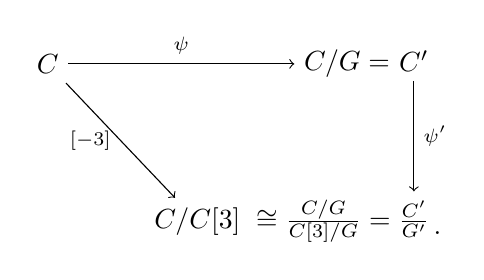
\begin{tikzpicture}[baseline=(current bounding box.center)]
          \node (LT) at (0, 2) {$C$}; 
          \node (MT) at (3.8, 2) {$C/G = $}; 
          \node (RT) at (4.65, 2.04) {$C'$}; 
          \node (LB) at (1.9, 0) {$C/C[3]$}; 
          \node (MB) at (3.5, 0) {$\cong \frac{C/G}{C[3]/G} = $}; 
          \node (RB) at (4.65, 0.025) {$\frac{C'}{G'}$}; 
          \node at (4.95, -0.15) {.}; 
          \draw [->] (LT) -- node [above] {$\scriptstyle \psi$} (MT); 
          \draw [->] (LT) -- node [left] {$\scriptstyle [-3]$} (LB); 
          \draw [->] (RT) -- node [right] {$\scriptstyle \psi'$} (RB); 
  \end{tikzpicture}
 \end{equation}
\end{prop}
\begin{proof}
 By \cite[2.4.2]{KM}, since $\Proj \s_3$ is connected, we need only show that the locus over which $\psi' \circ \psi = [-3]$ is not empty, 
 where by abuse of notation $[-3]$ denotes the map $[-3]$ on $C$ composed with the canonical isomorphism from $C/C[3]$ to $C'/G'$.  

 Recall from Section \ref{subsec:ec} that $C$ restricts to the supersingular locus $\BF_3$ as 
 \[
  C_0 \co y^2 + x y - y = x^3 - x^2.  
 \]
 By \isog{iii} both $\psi$ and $\psi'$ restrict as the 3-power Frobenius endomorphism $\psi_0$.   
 By \cite[2.6.3]{KM}, in the endomorphism ring of $C_0$, $\psi_0$ is a root of the polynomial 
 \begin{equation}
 \label{charpoly}
  X^2 - {\rm trace}(\psi_0) \cdot X + 3 
 \end{equation}
 with ${\rm trace}(\psi_0)$ an integer satisfying 
 \[
  \big( {\rm trace}(\psi_0) \big)^2 \leq 4 \cdot 3.  
 \]
 Moreover by \cite[Exercise 5.10a]{AEC}, since $C_0$ is supersingular, we have 
 \[
  {\rm trace}(\psi_0) \equiv 0 \md 3.  
 \]
 Thus ${\rm trace}(\psi_0) = 0$, 3, or $-3$.  
 We exclude the latter two possibilities by checking the action of $\psi_0$ at the 2-torsion point $(1,0)$.  
 It then follows from \eqref{charpoly} that $\psi_0 \circ \psi_0$ agrees with $[-3]$ on $C_0$ over $\BF_3$.  
\end{proof}

Analogous to \isog{iv}, let $\K'$ be the element in $\s_3$ such that $(\psi')^*$ sends $du$ to $\K' du$.  Note that $|\K'| = -6$.  

\begin{cor}
\label{cor:K'}
 The following relations hold in $\s_3$: 
 \[
  b^4 \K \K' + 3 = 0 
 \]
 and 
 \[
  \K' = -\K^3 + \frac{6}{b^2} ~ \K - \frac{a^2 - 8 b}{b^4}.  
 \]
\end{cor}
\begin{proof}
 The isogenies in \eqref{frob^2} induce maps on relative cotangent spaces at the identity.  
 By \isog{iv} we then have a commutative diagram 
 \begin{center}
 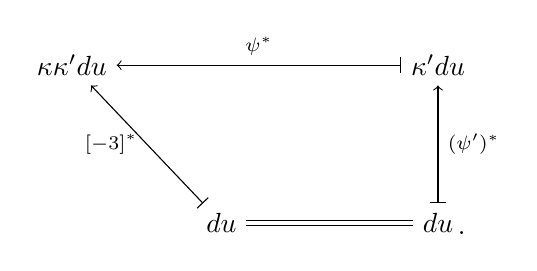
\begin{tikzpicture}
         \node (LT) at (0, 2) {$\K \K' du$}; 
         \node (RT) at (4.65, 2) {$\K' du$}; 
         \node (LB) at (1.9, 0) {$du$}; 
         \node (RB) at (4.65, 0) {$du$}; 
         \node at (4.95, -0.125) {.}; 
         \draw [|->] (RT) -- node [above] {$\scriptstyle \psi^*$} (LT); 
         \draw [|->] (LB) -- node [left] {$\scriptstyle [-3]^*$} (LT); 
         \draw [|->] (RB) -- node [right] {$\scriptstyle (\psi')^*$} (RT); 
         \draw [double distance=1.3pt] (LB) -- (RB); 
 \end{tikzpicture}
 \end{center}
 Thus for the first stated relation we need only show that $[3]^*$ sends $du$ to $3 du / b^4$.  

 For $i = 1$, 2, 3, and 4, let $Q_i$ be a generator for each of the four order-3 subgroups of $C$.  
 Each $Q_i$ can be chosen as $Q$ in \eqref{u'v'}, 
 and we denote the corresponding quantity $\K$ in \eqref{KL} by $\K_i$.  
 In view of \eqref{norm}, since $[3]$ has the same kernel as the isogeny $\Psi$ given by 
 \begin{equation*}
 \begin{split}
  u\big( \Psi(P) \big) \coloneqq & ~ u(P) \prod_{i=1}^4 \big( u(P-Q_i) \cdot u(P+Q_i) \big), \\
  v\big( \Psi(P) \big) \coloneqq & ~ v(P) \prod_{i=1}^4 \big( v(P-Q_i) \cdot v(P+Q_i) \big), 
 \end{split}
 \end{equation*}
 we have 
 \begin{equation}
 \label{s}
  [3]^* (du) = s \cdot \K_1 \K_2 \K_3 \K_4 \cdot du 
 \end{equation}
 where $s$ is a degree-0 unit in $\s$ coming from an automorphism of $C$ over $\s$.  
 In view of \eqref{W} we have 
 \[
  \K_1 \K_2 \K_3 \K_4 = -\frac{3}{b^4}.  
 \]
 We then compute that $s = -1$ by comparing the restrictions of the two sides of \eqref{s} to $S$ (\cf \eqref{S}): 
 $[3]^*$ becomes the multiplication-by-3 map, and $-3 / b^4$ becomes $-3$ (\cf \eqref{w}).  
 Thus $[3]^*$ sends $du$ to $3 du / b^4$.  

 The second stated relation follows by a computation from the first relation and $W(\K) = 0$ as in \isog{i}.  
\end{proof}

\begin{rmk}
\label{rmk:KK'}
 As noted in Remark \ref{rmk:K}, the (local) analog of $\K$ at the prime 2 coincides with the parameter $d$ in \cite[Section 3]{h2p2}.  
 In particular, with the notations there and the equation in \cite[Proposition 3.2]{tmf3}, 
 $d$ and $d'$ satisfy an analogous relation $b d d' + 2 = 0$ which locally reduces to $d d' + 2 = 0$ 
 (the analog of the factor $s$ in the proof of Corollary \ref{cor:K'} equals 1; \cf \cite[Theorem 2.5.7]{andoduke}).  
 These arise as examples of \cite[Lemma 3.21]{poonen}.  
\end{rmk}

\begin{rmk}
\label{rmk:K'}
 In view of \eqref{frob^2}, $-\psi'$ (composed with the canonical isomorphism on the target) 
 turns out to be the dual isogeny of $\psi$ (\cf the proof of \cite[2.9.4]{KM}).  
 If $G$ is the unique order-3 subgroup of $C$ in a formal neighborhood of the identity, 
 then 
 \[
  \K \equiv 0 \md 3 
 \]
 by Remark \ref{rmk:dmod3} and \eqref{K}.  
 Thus in view of Corollary \ref{cor:K'} and \eqref{H} we have 
 \[
  -\K' = \K^3 - \frac{6}{b^2} ~ \K + \frac{a^2 - 8 b}{b^4} \equiv \frac{H}{b^4} \md 3.  
 \]
 This congruence agrees with the interpretation of $H$ as defined by the tangent map of the Verschiebung isogeny over $\BF_3$ (\cf \cite[12.4.1]{KM}).  
\end{rmk}


\subsection{Individual power operations}

Let $A$ be a $K(2)$-local commutative $E$-algebra.  
By \cite[3.23]{cong} and Corollary \ref{cor:psi3}, 
we have a total power operation 
\[
 \p \co A_0 \to A_0 \otimes_{E_0} (E^0 B\Sigma_3 / I) \cong A_0 [\A] \big/ \big( w(\A) \big).  
\]
We also have a composite of total power operations 
\begin{equation}
\label{psi3^2}
\begin{split}
 A_0 \stackrel{\p}{\longrightarrow} A_0 \otimes_{E_0} (E^0 B\Sigma_3 / I) \stackrel{\p}{\longrightarrow} 
 & ~ \big( A_0 \otimes_{E_0} (E^0 B\Sigma_3 / I) \big) \tensor[^\p]{\otimes}{_{E_0 [\A]}} (E^0 B\Sigma_3 / I) \\
 \cong & ~ \Big( A_0 [\A] \big/ \big( w(\A) \big) \Big) \tensor[^\p]{\otimes}{_{E_0 [\A]}} \Big( E^0 [\A] \big/ \big( w(\A) \big) \Big) 
\end{split}
\end{equation}
where the elements in the target $M \tensor[^\p]{\otimes}{_R} N$ are subject to the equivalence relation (as well as other ones in a usual tensor product) 
\[
 m \otimes (r \cdot n) \sim \big( m \cdot \p(r) \big) \otimes n 
\]
for $m \in M$, $n \in N$, and $r \in R$ with 
\[
 \p(\A) = -\A^3 + 6 \A - h + 9 
\]
by Corollary \ref{cor:K'}.  

\begin{defn}
 Define the {\em individual power operations} 
 \[
  Q_k \co A_0 \to A_0 
 \]
 for $k = 0$, 1, 2, and 3 by 
 \begin{equation}
 \label{Q_k}
  \p (x) = Q_0(x) + Q_1(x) \A + Q_2(x) \A^2 + Q_3(x) \A^3.  
 \end{equation}
\end{defn}

\begin{prop}
\label{prop:Q}
 The following relations hold among the individual power operations $Q_0$, $Q_1$, $Q_2$, and $Q_3$: 
 \begin{enumerate}[(i)]
  \item $Q_0(1) = 1, \quad Q_1(1) = Q_2(1) = Q_3(1) = 0;$ \label{Q(i)}

  \item $Q_k(x+y) = Q_k(x) + Q_k(y) \text{~for all~} k;$ \label{Q(ii)}

  \item {\em Commutation relations} \label{Q(iii)}
  \begin{equation*}
  \begin{split}
   Q_0(h x) = & ~ (h^3 - 27 h^2 + 201 h - 342) Q_0(x) + (3 h^2 - 54 h + 171) Q_1(x) \qquad \qquad \\
              & + (9 h - 81) Q_2(x) + 24 Q_3(x), \\
   Q_1(h x) = & ~ (-6 h^2 + 108 h - 334) Q_0(x) + (-18 h + 171) Q_1(x) + (-72) Q_2(x) \\
              & + (h - 9) Q_3(x), \\
   Q_2(h x) = & ~ (3 h - 27) Q_0(x) + 8 Q_1(x) + 9 Q_2(x) + (-24) Q_3(x), \\
   Q_3(h x) = & ~ (h^2 - 18 h + 57) Q_0(x) + (3 h - 27) Q_1(x) + 8 Q_2(x) + 9 Q_3(x), \\
   Q_0(c x) = & ~ (c^3 - 12 c + 12 c^{-1}) Q_0(x) + (3 c - 12 c^{-1}) Q_1(x) + (12 c^{-1}) Q_2(x) \\
              & + (-12 c^{-1}) Q_3(x), \\
   Q_1(c x) = & ~ (-6 c + 20 c^{-1}) Q_0(x) + (-20 c^{-1}) Q_1(x) + (- c + 20 c^{-1}) Q_2(x) \\
              & + (4 c - 20 c^{-1}) Q_3(x), \\
   Q_2(c x) = & ~ (4 c^{-1}) Q_0(x) + (-4 c^{-1}) Q_1(x) + (4 c^{-1}) Q_2(x) + (- c - 4 c^{-1}) Q_3(x), \\
   Q_3(c x) = & ~ (c - 4 c^{-1}) Q_0(x) + (4 c^{-1}) Q_1(x) + (-4 c^{-1}) Q_2(x) + (4 c^{-1}) Q_3(x), \\
   Q_k(i x) = & ~ (-i) Q_k(x) \text{~for all~} k; \\
  \end{split}
  \end{equation*}

  \item {\em Adem relations} \label{Q(iv)}
  \begin{equation*}
  \begin{split}
   Q_1Q_0(x) = & ~ (-6) Q_0Q_1(x) + 3 Q_2Q_1(x) + (6 h - 54) Q_0Q_2(x) + 18 Q_1Q_2(x) \\
               & + (-9) Q_3Q_2(x) + (-6 h^2 + 108 h - 369) Q_0Q_3(x) \\
               & + (-18 h + 162) Q_1Q_3(x) + (-54) Q_2Q_3(x), \\
   Q_2Q_0(x) = & ~ 3 Q_3Q_1(x) + (-3) Q_0Q_2(x) + (3 h - 27) Q_0Q_3(x) + 9 Q_1Q_3(x), \qquad \qquad \\
   Q_3Q_0(x) = & ~ Q_0Q_1(x) + (-h + 9) Q_0Q_2(x) + (-3) Q_1Q_2(x) \\
               & + (h^2 - 18 h + 63) Q_0Q_3(x) + (3 h - 27) Q_1Q_3(x) + 9 Q_2Q_3(x); 
  \end{split}
  \end{equation*}

  \item {\em Cartan formulas} \label{Q(v)}
  \begin{equation*}
  \begin{split}
   Q_0(xy) = & ~ Q_0(x) Q_0(y) + 3 \big( Q_3(x) Q_1(y) + Q_2(x) Q_2(y) + Q_1(x) Q_3(y) \big) \\
             & + 18 Q_3(x) Q_3(y), \\
   Q_1(xy) = & ~ \big( Q_1(x) Q_0(y) + Q_0(x) Q_1(y) \big) \\
             & + (-h + 9) \big( Q_3(x) Q_1(y) + Q_2(x) Q_2(y) + Q_1(x) Q_3(y) \big) \\
             & + 3 \big( Q_3(x) Q_2(y) + Q_2(x) Q_3(y) \big) + (-6 h + 54) Q_3(x) Q_3(y), \qquad \qquad \qquad
  \end{split}
  \end{equation*}
  \begin{equation*}
  \begin{split}
   Q_2(xy) = & ~ \big( Q_2(x) Q_0(y) + Q_1(x) Q_1(y) + Q_0(x) Q_2(y) \big) \\
             & + 6 \big( Q_3(x) Q_1(y) + Q_2(x) Q_2(y) + Q_1(x) Q_3(y) \big) \\
             & + (-h + 9) \big( Q_3(x) Q_2(y) + Q_2(x) Q_3(y) \big) + 39 Q_3(x) Q_3(y), \\
   Q_3(xy) = & ~ \big( Q_3(x) Q_0(y) + Q_2(x) Q_1(y) + Q_1(x) Q_2(y) + Q_0(x) Q_3(y) \big) \qquad \qquad \qquad \\
             & + 6 \big( Q_3(x) Q_2(y) + Q_2(x) Q_3(y) \big) + (-h + 9) Q_3(x) Q_3(y); 
  \end{split}
  \end{equation*}

  \item {\em Frobenius congruence} \label{Q(vi)}
  \begin{equation*}
   Q_0(x) \equiv x^3 \md 3.  \qquad \qquad \qquad \qquad \qquad \qquad \qquad \qquad \qquad \qquad \qquad \qquad
  \end{equation*}
 \end{enumerate}
\end{prop}
\begin{proof}
 The relations in \eqref{Q(i)}, \eqref{Q(ii)}, \eqref{Q(iii)}, and \eqref{Q(v)} follow computationally from 
 the fact that $\p$ is a ring homomorphism together with the formulas in Corollary \ref{cor:psi3}.  

 For \eqref{Q(iv)}, there is a canonical isomorphism $C/C[3] \cong C$ of elliptic curves.  
 Given the correspondence between deformations of Frobenius and power operations in \cite[Theorem B]{cong}, 
 the commutativity of \eqref{frob^2} then implies that the composite \eqref{psi3^2} lands in $A_0$.  In terms of formulas, we have 
 \begin{equation*}
 \begin{split}
  \p \big( \p(x) \big) = & ~ \p \big( Q_0(x) + Q_1(x) \A + Q_2(x) \A^2 + Q_3(x) \A^3 \big) \\
                       = & ~ \sum_{k = 0}^3 \p \big( Q_k(x) \big) \big( \p(\A) \big)^k \\
                       = & ~ \sum_{k = 0}^3 \sum_{j = 0}^3 Q_jQ_k(x) \A^j (-\A^3 + 6 \A - h + 9)^k \\
                  \equiv & ~ \Psi_0(x) + \Psi_1(x) \A + \Psi_2(x) \A^2 + \Psi_3(x) \A^3 \md \big( w(\A) \big) 
 \end{split}
 \end{equation*}
 where each $\Psi_i$ is an $E_0$-linear combination of the $Q_jQ_k$'s.  
 The vanishing of $\Psi_1(x)$, $\Psi_2(x)$, and $\Psi_3(x)$ gives the three relations in \eqref{Q(iv)}.  

 For \eqref{Q(vi)}, by \cite[Propositions 3.25 and 10.5]{cong} we have 
 \[
  \p(x) \equiv x^3 \md 3.  
 \]
 In view of \eqref{Amod3}, the congruence in \eqref{Q(vi)} then follows from \eqref{Q_k}.  
\end{proof}

\begin{ex}
\label{ex}
 We have $E^0 S^2 \cong \BZ_9 \llbracket h \rrbracket [u] / (u^2)$.  
 By definition of $\K$ in \eqref{KL}, the $Q_k$'s act canonically on $u \in E^0 S^2$: 
 \[
  Q_k(u) = \left\{
  \begin{array}{ll}
    u,  & \quad {\rm if}~k = 1, \\
    0,  & \quad {\rm if}~k \neq 1.  \\
  \end{array}
  \right.
 \]
 We then get the values of the $Q_k$'s on elements in $E^0 S^2$ from \q{i}-\eqref{Q(iii)}.  
\end{ex}


\subsection{The \DL algebra}

\begin{defn}
\label{def:go}
 \mbox{}
 \begin{enumerate}[(i)]
  \item \label{go(i)} Let $i$ be an element generating $\BZ_9$ over $\BZ_3$ with $i^2 = -1$.  
  Define $\g$ to be the associative ring generated over $\BZ_9 \llbracket h \rrbracket$ 
  by elements $q_0$, $q_1$, $q_2$, and $q_3$ subject to the following relations: 
  the $q_k$'s commute with elements in $\BZ_3 \subset \BZ_9 \llbracket h \rrbracket$, 
  and satisfy {\em commutation relations} 
  \begin{equation*}
  \begin{split}
   q_0 h = & ~ (h^3 - 27 h^2 + 201 h - 342) q_0 + (3 h^2 - 54 h + 171) q_1 + (9 h - 81) q_2 \\
           & + 24 q_3, \\
   q_1 h = & ~ (-6 h^2 + 108 h - 334) q_0 + (-18 h + 171) q_1 + (-72) q_2 + (h - 9) q_3, \\
   q_2 h = & ~ (3 h - 27) q_0 + 8 q_1 + 9 q_2 + (-24) q_3, \\
   q_3 h = & ~ (h^2 - 18 h + 57) q_0 + (3 h - 27) q_1 + 8 q_2 + 9 q_3, \\
   q_k i = & ~ (-i) q_k \text{~for all~} k, 
  \end{split}
  \end{equation*}
  and {\em Adem relations} 
  \begin{equation*}
  \begin{split}
   q_1q_0 = & ~ (-6) q_0q_1 + 3 q_2q_1 + (6 h - 54) q_0q_2 + 18 q_1q_2 + (-9) q_3q_2 \\
            & + (-6 h^2 + 108 h - 369) q_0q_3 + (-18 h + 162) q_1q_3 + (-54) q_2q_3, \quad~~ \\
   q_2q_0 = & ~ 3 q_3q_1 + (-3) q_0q_2 + (3 h - 27) q_0q_3 + 9 q_1q_3, \\
   q_3q_0 = & ~ q_0q_1 + (-h + 9) q_0q_2 + (-3) q_1q_2 + (h^2 - 18 h + 63) q_0q_3 \\
            & + (3 h - 27) q_1q_3 + 9 q_2q_3.  
  \end{split}
  \end{equation*}

  \item \label{go(ii)} Write $\omega \coloneqq \pi_2 E$ which is the kernel of $E^0 S^2 \to E^0$ with $E^0 S^2 \cong \BZ_9 \llbracket h \rrbracket [u] / (u^2)$.  
  Define $\omega$ as a $\g$-module in the sense of \cite[2.2]{h2p2} with one generator $u$ by 
  \[
   q_k \cdot u = \left\{
   \begin{array}{ll}
     u,  & \quad {\rm if}~k = 1, \\
     0,  & \quad {\rm if}~k \neq 1.  \\
   \end{array}
   \right.
  \]
 \end{enumerate}
\end{defn}

\begin{rmk}
\label{rmk:rank}
 In \go{i}, an element $r \in \BZ_9 \llbracket h \rrbracket \cong E_0$ 
 corresponds to the multiplication-by-$r$ operation (\cf \cite[Proposition 6.4]{cong}), 
 and each $q_k$ corresponds to the individual power operation $Q_k$ (also compare \go{ii} and Example \ref{ex}).  
 Under this correspondence, the relations in \q{ii}-\eqref{Q(v)}  describe explicitly the structure of $\g$ as 
 that of a {\em graded twisted bialgebra over $E_0$} in the sense of \cite[Section 5]{cong}.  
 The grading of $\g$ comes from the number of the $q_k$'s in a monomial: for example, commutation relations are in degree 1, and Adem relations are in degree 2.  
 Under these relations, $\g$ has an {\em admissible basis}: it is free as a left $E_0$-module on the elements of the form 
 \[
  q_0^m q_{k_1} \cdots q_{k_n} 
 \]
 where $m, n \geq 0$ ($n = 0$ gives $q_0^m$), and $k_i = 1$, 2, or 3.  
 If we write $\g[d]$ for the degree-$d$ part of $\g$, then $\g[d]$ is of rank $1 + 3 + \cdots + 3^d$.  
\end{rmk}

We now identify $\g$ with the \DL algebra of power operations on $K(2)$-local commutative $E$-algebras.  

\begin{thm}
\label{thm:gamma}
 Let $A$ be a $K(2)$-local commutative $E$-algebra.  
 Let $\g$ be the graded twisted bialgebra over $E_0$, and $\omega$ be the $\g$-module in Definition \ref{def:go}.  
 Then $A_*$ is an {\em $\omega$-twisted $\BZ/2$-graded amplified $\g$-ring} in the sense of \cite[Section 2]{cong} and \cite[2.5 and 2.6]{h2p2}.  In particular, 
 \[
  \pi_* L_{K(2)} \BP_E (\Sigma^d E) \cong \big( F_d \big)_{(3,h)}^\wedge 
 \]
 where $F_d$ is the free $\omega$-twisted $\BZ/2$-graded amplified $\g$-ring with one generator in degree $d$.  
\end{thm}
Formulas for $\g$ aside, this result is due to Rezk \cite{cong, h2p2}.  
\begin{proof}
 Let $\G$ be the graded twisted bialgebra of power operations on $E_0$ in \cite[Section 6]{cong}.  
 We need only identify $\G$ with $\g$.  

 There is a direct sum decomposition $\G = \bigoplus_{d \geq 0} \G[d]$ 
 where the summands come from the completed $E$-homology of $B\Sigma_{3^d}$ (\cf \cite[6.2]{cong}).  
 As in Remark \ref{rmk:rank}, we have a degree-preserving ring homomorphism 
 \[
  \phi \co \g \to \G, \qquad q_k \mapsto Q_k 
 \]
 which is an isomorphism in degrees 0 and 1.  
 We need to show that $\phi$ is both surjective and injective in all degrees.  

 For the surjectivity of $\phi$, we use a transfer argument.  
 We have 
 \[
  \nu_3(|\Sigma_3^{\wr d}|) = \nu_3(|\Sigma_{3^d}|) = (3^d - 1) / 2 
 \]
 where $\nu_3(-)$ is the 3-adic valuation, and $(-)^{\wr d}$ is the $d$-fold wreath product.  
 Thus following the proof of \cite[Proposition 3.17]{cong}, 
 we see that $\G$ is generated in degree 1, and hence $\phi$ is surjective.  

 By Remark \ref{rmk:rank} and (the $E_0$-linear dual of) \cite[Theorem 1.1]{Str98}, 
 $\g[d]$ and $\G[d]$ are of the same rank $1 + 3 + \cdots + 3^d$ as free modules over $E_0$.  
 Hence $\phi$ is also injective.  
\end{proof}


\section{$K(1)$-local power operations}
\label{sec:K(1)}

Let $F \coloneqq L_{K(1)} E$ be the $K(1)$-localization of $E$.  
The relationship between the power operation on $E^0$ in Corollary \ref{cor:psi3} 
and $K(1)$-local power operations on $F^0$ (\cf \cite[Section 3]{hopkins} and \cite[Section IX.3]{H_infty}) is as follows: 
\begin{center}
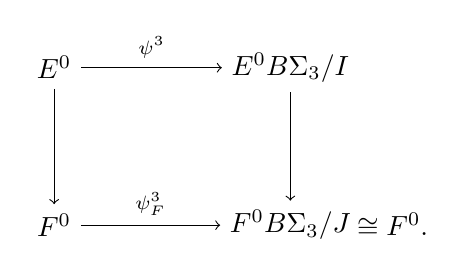
\begin{tikzpicture}
        \node (LT) at (0, 2) {$E^0$}; 
        \node (RT) at (3, 2) {$E^0 B\Sigma_3 / I$}; 
        \node (LB) at (0, 0) {$F^0$}; 
        \node (MB) at (3, 0) {$F^0 B\Sigma_3 / J$}; 
        \node (RB) at (4.3, 0) {$\cong F^0.  $}; 
        \draw [->] (LT) -- node [above] {$\scriptstyle \p$} (RT); 
        \draw [->] (LT) -- (LB); 
        \draw [->] (RT) -- (MB); 
        \draw [->] (LB) -- node [above] {$\scriptstyle \psi_F^3$} (MB); 
\end{tikzpicture}
\end{center}
Here $\psi_F^3$ is the $K(1)$-local power operation induced by $\p$, and $J \cong F^0 \otimes_{E^0} I$ is the transfer ideal (\cf \eqref{transfer}).  
Recall from \isog{i}, \eqref{S_3}, and Corollary \ref{cor:psi3} that $\p$ arises from the universal degree-3 isogeny 
which is parametrized by the ring $\s_3$ with 
\[
 \big( S_3 \big)_{(3,h)}^\wedge \cong E^0 B\Sigma_3 / I.  
\]
The vertical maps are induced by the $K(1)$-localization $E \to F$.  In terms of 
homotopy groups, this is obtained by inverting the generator $h$ 
and completing at the prime 3 (\cf \cite[Corollary 1.5.5]{hovey}): 
\[
 E_* = \BZ_9 \llbracket h \rrbracket [u^{\pm1}] \qquad \ad \qquad F_* = \BZ_9 \llbracket h \rrbracket [h^{-1}]_3^\wedge [u^{\pm1}] 
\]
with 
\[
 F_0 = \BZ_9 (\!(h)\!)_3^\wedge = \left.\left\{\sum_{n = -\infty}^{\infty} k_n h^n~\right|~k_n \in \BZ_9, \lim_{n \to -\infty} k_n = 0\right\}.  
\]
The formal group $\HC$ over $E^0$ has a unique order-3 subgroup after being pulled back to $F^0$ (\cf Remark \ref{rmk:dmod3}), 
and the map 
\[
 E^0 B\Sigma_3 / I \to F^0 B\Sigma_3 / J \cong F^0 
\]
classifies this subgroup.  Along the base change 
\[
 E^0 B\Sigma_3 / I \to F^0 \otimes_{E^0} (E^0 B\Sigma_3 / I) \cong (F^0 \otimes_{E^0} E^0 B\Sigma_3) / J \cong F^0 B\Sigma_3 / J, 
\]
the special fiber of the 3-divisible group of $\HC$ which consists solely of a formal component may split into formal and \'etale components.  
We want to take the formal component so as to keep track of the unique order-3 subgroup of the formal group over $F^0$.  
This subgroup gives rise to the $K(1)$-local power operation $\psi_F^3$.  

Recall from \eqref{S_3} that $S_3 = S[\A] \big/ \big( w(\A) \big)$.  Since 
\[
 w(\A) = \A^4 - 6 \A^2 + (h - 9) \A - 3 \equiv \A (\A^3 + h) \md 3, 
\]
the equation $w(\A) = 0$ has a unique root $\A = 0$ in $\BF_9 (\!(h)\!)$ (\cf \eqref{Amod3}).  
By Hensel's lemma this unique root lifts to a root in $\BZ_9 (\!(h)\!)_3^\wedge$; 
it corresponds to the unique order-3 subgroup of $\HC$ over $F^0$.  
Plugging this specific value of $\A$ into the formulas for $\p$ in Corollary \ref{cor:psi3}, we then get an endomorphism of the ring $F^0$.  
This endomorphism is the $K(1)$-local power operation $\psi_F^3$.  

Explicitly, with $h$ invertible in $F^0$, we solve for $\A$ from $w(\A) = 0$ by first writing 
\[
 \A = (3 + 6 \A^2 - \A^4) / (h - 9) = (3 + 6 \A^2 - \A^4) \sum_{n = 1}^\infty 9^{n-1} h^{-n} 
\]
and then substituting this equation into itself recursively.  We plug the power series expansion for $\A$ into $\p(h)$ and get 
\[
 \psi_F^3(h) = h^3 - 27 h^2 + 183 h - 180 + 186 h^{-1} + 1674 h^{-2} + (\text{lower-degree terms}).  ~~~
\]
Similarly, writing $h$ as $c^2 + 1$ in $w(\A) = 0$, we solve for $\A$ in terms of $c$ and get 
\[
 \psi_F^3(c) = c^3 - 12 c - 6 c^{-1} - 84 c^{-3} - 933 c^{-5} - 10956 c^{-7} + (\text{lower-degree terms}).  
\]


\appendix
\section*{Appendices}

Here we list long formulas whose appearance in the main body might affect readability.  
The calculations involve power series expansions and manipulations of long polynomials with large coefficients 
(division, factorization, and finding greatest common divisors).  
They are done using the software {\em Wolfram Mathematica 8}.  
The commands \texttt{Reduce} and \texttt{Solve} are used to extract relations out of given identities.  


\section{Formulas in the proof of Proposition \ref{prop:tors}}
\label{apx:tors}

\begin{equation*}
\begin{split}
 \Tf(u) = & -\frac{u^4}{a^2 b} \big( b^4 u^8 + 3 a b^3 u^7 + 3 a^2 b^2 u^6 + (a^3 b + 7 a b^2) u^5 + (6 a^2 b - 6 b^2) u^4 \qquad~~ \\
          & + 9 a b u^3 + (-a^2 + 8 b) u^2 - 3 a u - 3 \big), \\
 Q_1(v) = & ~ a b^2 v^2 + (b^2 d^2 + 2 a b d - b) v + \frac{b^2 d^4}{a} + 2 b d^3 + a d^2 - \frac{2 b d^2}{a} - d + \frac{1}{a}, 
\end{split}
\end{equation*}
\begin{equation*}
\begin{split}
 R_1(v) = & ~ (\frac{b^3 d^6}{a} + 2 b^2 d^5 + a b d^4 - \frac{3 b^2 d^4}{a} + 2 b d^3 + \frac{3 b d^2}{a} - \frac{1}{a}) v + \frac{b^2 d^7}{a} + 2 b d^6 \\
          & + a d^5 - \frac{2 b d^5}{a} + 2 d^4 + \frac{d^3}{a}, \\
 Q_2(v) = & ~ \frac{a}{(b^3 d^6 + 2 a b^2 d^5 + a^2 b d^4 - 3 b^2 d^4 + 2 a b d^3 + 3 b d^2 - 1)^2} \big( (a b^4 d^6 + 2 a^2 b^3 d^5 \\
          & + a^3 b^2 d^4 - 3 a b^3 d^4 + 2 a^2 b^2 d^3 + 3 a b^2 d^2 - a b) v - b^4 d^8 - 2 a b^3 d^7 - a^2 b^2 d^6 \\
          & + 4 b^3 d^6 - a b^2 d^5 + a^2 b d^4 - 6 b^2 d^4 + 4 a b d^3 + 4 b d^2 - a d - 1 \big), \\
 R_2 = & - \frac{a d^4}{(b^3 d^6 + 2 a b^2 d^5 + a^2 b d^4 - 3 b^2 d^4 + 2 a b d^3 + 3 b d^2 - 1)^2} (b^4 d^8 + 3 a b^3 d^7 \\
       & + 3 a^2 b^2 d^6 + a^3 b d^5 + 7 a b^2 d^5 + 6 a^2 b d^4 - 6 b^2 d^4 + 9 a b d^3 - a^2 d^2 + 8 b d^2 \\
       & - 3 a d - 3), \\
 K(u) = & ~ \frac{b^3 u^6}{a} + 2 b^2 u^5 + (a b - \frac{3 b^2}{a}) u^4 + 2 b u^3 + \frac{3 b u^2}{a} - \frac{1}{a}, \\
 L(u) = & ~ \frac{b^2 u^7}{a} + 2 b u^6 + (a - \frac{2 b}{a}) u^5 + 2 u^4 + \frac{u^3}{a}, \\
 M(u) = & ~ \frac{b}{a^2 (a^2 - 16 b)^2} \big( (10 a^3 b^3 - 112 a b^4) u^5 + (19 a^4 b^2 - 217 a^2 b^3 - 16 b^4) u^4 \\
        & + (8 a^5 b - 126 a^3 b^2 + 304 a b^3) u^3 + (-a^6 + 34 a^4 b -266 a^2 b^2 +32 b^3) u^2 \\
        & + (28 a^3 b - 384 a b^2) u - 4 a^4 + 51 a^2 b - 16 b^2 \big), \\
 N(u) = & -\frac{1}{a (a^2 - 16 b)^2} \big( (10 a^3 b^5 - 112 a b^6) u^7 + (29 a^4 b^4 - 329 a^2 b^5 - 16 b^6) u^6 \\
        & + (27 a^5 b^3 - 313 a^3 b^4 - 48 a b^5 ) u^5 + (7 a^6 b^2 - 15 a^4 b^3 - 837 a^2 b^4 - 16 b^5) u^4 \\
        & + (-a^7 b + 66 a^5 b^2 - 714 a^3 b^3 + 528 a b^4) u^3 + (-4 a^6 b + 137 a^4 b^2 \\
        & - 1147 a^2 b^3 + 80 b^4) u^2 + (-12 a^5 b + 237 a^3 b^2 - 1200 a b^3) u + a^6 - 44 a^4 b \\
        & + 409 a^2 b^2 - 48 b^3 \big).  
\end{split}
\end{equation*}


\section{Formulas in the proof of Proposition \ref{prop:isog}}
\label{apx:isog}

The power series expansion of $v$ in terms of $u$ up to $u^{12}$ is 
\begin{equation*}
\begin{split}
 v = & ~ u^3 - a u^4 + (a^2 + b) u^5 + (-a^3 - 3 a b) u^6 + (a^4 + 6 a^2 b + b^2) u^7 + (-a^5 - 10 a^3 b \\
     & - 6 a b^2) u^8 + (a^6 + 15 a^4 b + 20 a^2 b^2 + b^3) u^9 + (-a^7 - 21 a^5 b - 50 a^3 b^2 \\
     & - 10 a b^3) u^{10} + (a^8 + 28 a^6 b + 105 a^4 b^2 + 50 a^2 b^3 + b^4) u^{11} + (-a^9 - 36 a^7 b \\
     & - 196 a^5 b^2 - 175 a^3 b^3 - 15 a b^4) u^{12}.  
\end{split}
\end{equation*}

The group law on $C$ satisfies: 
\begin{itemize}
 \item given $P(u,v)$, the coordinates of $-P$ are 
 \[
  \left( -\frac{v}{u (u + b v)},-\frac{v^2}{u^2 (u + b v)} \right); 
 \]

 \item given $P_1(u_1,v_1)$ and $P_2(u_2,v_2)$, the coordinates of $-(P_1 + P_2)$ are 
 \[
  u_3 \coloneqq a k - \frac{b m}{1 + b k} - u_1 - u_2 \qquad \ad \qquad v_3 \coloneqq k u_3 + m 
 \]
 where 
 \[
  k = \frac{v_1 - v_2}{u_1 - u_2} \qquad \ad \qquad m = \frac{u_1 v_2 - u_2 v_1}{u_1 - u_2}.  
 \]
\end{itemize}
Given $P(u,v)$ and $Q(d,e)$, with the above notations and formulas, 
\begin{itemize}
 \item set 
 \[
  (u_1,v_1) = \left( -\frac{v}{u (u + b v)},-\frac{v^2}{u^2 (u + b v)} \right) \qquad \ad \qquad (u_2,v_2) = (d,e) 
 \]
 so that 
 \[
  P - Q = (u_3,v_3); 
 \]

 \item set 
 \[
  (u_1,v_1) = (u,v) \qquad \ad \qquad (u_2,v_2) = (d,e) 
 \]
 so that 
 \[
  P + Q = \left( -\frac{v_3}{u_3 (u_3 + b v_3)},-\frac{v_3^2}{u_3^2 (u_3 + b v_3)} \right).  
 \]
\end{itemize}
Plugging the coordinates of $P - Q$ and $P + Q$ into \eqref{u'v'}, and in view of \eqref{f}, 
we then have in \eqref{KL} 
\begin{equation*}
\begin{split}
      \K = & -\frac{1}{a^2 - 16 b} \big( a b^3 d^7 + (3 a^2 b^2 - 2 b^3) d^6 + (3 a^3 b - 6 a b^2) d^5 + (a^4 + a^2 b + 2 b^2) d^4 \\
           & + (4 a^3 - 15 a b) d^3 + (a^2 + 2 b) d^2 - 12 a d - 18 \big), \\
 \lambda = & -\frac{1}{a^2 b^2 (a^2 - 16 b)} \big( (a^3  b^3 - 11 a b^4) d^7 + (3 a^4 b^2 - 33 a^2 b^3 - 4 b^4) d^6 + (3 a^5 b \\
           & - 33 a^3 b^2 - 15 a b^3) d^5 + (a^6 - 4 a^4 b - 96 a^2 b^2 - 4 b^3) d^4 + (6 a^5 - 80 a^3 b \\
           & + 31 a b^2) d^3 + (10 a^4 - 153 a^2 b + 20 b^2) d^2 + (3 a^3 - 117 a b) d - 6 a^2 - 12 b \big).  
\end{split}
\end{equation*}
More extended power series expansions in $u$ for $u'$ (up to $u^6$) and $v'$ (up to $u^9$) are needed in \eqref{KL} to determine the coefficients in the equation of $C'$: 
\begin{equation*}
\begin{split}
 u' = & -\frac{1}{a^2 - 16 b} \big( (a b^3 d^7 + 3 a^2 b^2 d^6 - 2 b^3 d^6 + 3 a^3 b d^5 - 6 a b^2 d^5 + a^4 d^4 + a^2 b d^4 \quad~~~ \\
      & + 2 b^2 d^4 + 4 a^3 d^3 - 15 a b d^3 + a^2 d^2 + 2 b d^2 - 12 a d - 18) u + (-a^2 b^3 d^7 
\end{split}
\end{equation*}
\begin{equation*}
\begin{split}
      & + 12 b^4 d^7 - 3 a^3 b^2 d^6 + 36 a b^3 d^6 - 3 a^4 b d^5 + 36 a^2 b^2 d^5 + 4 b^3 d^5 - a^5 d^4 \\
      & + 5 a^3 b d^4 + 94 a b^2 d^4 - 6 a^4 d^3 + 85 a^2 b d^3 - 76 b^2 d^3 - 9 a^3 d^2 + 136 a b d^2 + 60 b d \\
      & + 6 a) u^2 + (a^3 b^3 d^7 - 17 a b^4 d^7 + 3 a^4 b^2 d^6 - 50 a^2 b^3 d^6 - 8 b^4 d^6 + 3 a^5 b d^5 \\
      & - 48 a^3 b^2 d^5 - 27 a b^3 d^5 + a^6 d^4 - 7 a^4 b d^4 - 150 a^2 b^2 d^4 - 16 b^3 d^4 + 7 a^5 d^3 \\
      & - 113 a^3 b d^3 + 9 a b^2 d^3 + 16 a^4 d^2 - 258 a^2 b d^2 + 56 b^2 d^2 + 15 a^3 d - 237 a b d \\
      & + 2 a^2 - 32 b) u^3 + (-a^4 b^3 d^7 + 16 a^2 b^4 d^7 + 12 b^5 d^7 - 3 a^5 b^2 d^6 + 46 a^3 b^3 d^6 \\
      & + 64 a b^4 d^6 - 3 a^6 b d^5 + 42 a^4 b^2 d^5 + 121 a^2 b^3 d^5 + 4 b^4 d^5 - a^7 d^4 + 3 a^5 b d^4 \\
      & + 209 a^3 b^2 d^4 + 122 a b^3 d^4 - 8 a^6 d^3 + 114 a^4 b d^3 + 248 a^2 b^2 d^3 - 76 b^3 d^3 \\
      & - 24 a^5 d^2 + 384 a^3 b d^2 - 4 a b^2 d^2 - 33 a^4 d + 519 a^2 b d + 60 b^2 d - 18 a^3 \\
      & + 282 a b) u^4 + (a^5 b^3 d^7 - 9 a^3 b^4 d^7 - 117 a b^5 d^7 + 3 a^6 b^2 d^6 - 24 a^4 b^3 d^6 \\
      & - 396 a^2 b^4 d^6 - 24 b^5 d^6 + 3 a^7 b d^5 - 18 a^5 b^2 d^5 - 484 a^3 b^3 d^5 - 111 a b^4 d^5 + a^8 d^4 \\
      & + 7 a^6 b d^4 - 307 a^4 b^2 d^4 - 1038 a^2 b^3 d^4 + 9 a^7 d^3 - 73 a^5 b d^3 - 1181 a^3 b^2 d^3 \\
      & + 573 a b^3 d^3 + 33 a^6 d^2 - 451 a^4 b d^2 - 1236 a^2 b^2 d^2 + 72 b^3 d^2 + 54 a^5 d \\
      & - 807 a^3 b d - 873 a b^2 d + 36 a^4 - 570 a^2 b - 48 b^2) u^5 + (-a^6 b^3 d^7 - 5 a^4 b^4 d^7 \\
      & + 337 a^2 b^5 d^7 + 12 b^6 d^7 - 3 a^7 b^2 d^6 - 19 a^5 b^3 d^6 + 1064 a^3 b^4 d^6 + 204 a b^5 d^6 \\
      & - 3 a^8 b d^5 - 27 a^6 b^2 d^5 + 1164 a^4 b^3 d^5 + 638 a^2 b^4 d^5 + 4 b^5 d^5 - a^9 d^4 - 24 a^7 b d^4 \\
      & + 441 a^5 b^2 d^4 + 3195 a^3 b^3 d^4 + 182 a b^4 d^4 - 10 a^8 d^3 - 22 a^6 b d^3 + 2956 a^4 b^2 d^3 \\
      & - 645 a^2 b^3 d^3 - 76 b^4 d^3 - 43 a^7 d^2 + 403 a^5 b d^2 + 4594 a^3 b^2 d^2 - 544 a b^3 d^2 \\
      & - 78 a^6 d + 996 a^4 b d + 4014 a^2 b^2 d + 60 b^3 d - 57 a^5 + 852 a^3 b + 942 a b^2) u^6 \big), \\
 v' = & -\frac{1}{a^2 b^2 (a^2 - 16 b)} \big( (a^3 b^3 d^7 - 11 a b^4 d^7 + 3 a^4 b^2 d^6 - 33 a^2 b^3 d^6 - 4 b^4 d^6 \\
      & + 3 a^5 b d^5 - 33 a^3 b^2 d^5 - 15 a b^3 d^5 + a^6 d^4 - 4 a^4 b d^4 - 96 a^2 b^2 d^4 - 4 b^3 d^4 \\
      & + 6 a^5 d^3 - 80 a^3 b d^3 + 31 a b^2 d^3 + 10 a^4 d^2 - 153 a^2 b d^2 + 20 b^2 d^2 + 3 a^3 d \\
      & - 117 a b d - 6 a^2 - 12 b) u^3 + (-2 a^4 b^3 d^7 + 28 a^2 b^4 d^7 - 6 a^5 b^2 d^6 + 82 a^3 b^3 d^6 \\
      & + 28 a b^4 d^6 - 6 a^6 b d^5 + 78 a^4 b^2 d^5 + 90 a^2 b^3 d^5 - 2 a^7 d^4 + 8 a^5 b d^4 + 294 a^3 b^2 d^4 \\
      & + 20 a b^3 d^4 - 14 a^6 d^3 + 202 a^4 b d^3 + 72 a^2 b^2 d^3 - 32 a^5 d^2 + 510 a^3 b d^2 \\
      & - 124 a b^2 d^2 - 30 a^4 d + 546 a^2 b d - 6 a^3 + 204 a b) u^4 + (3 a^5 b^3 d^7 - 38 a^3 b^4 d^7 \\
      & - 107 a b^5 d^7 + 9 a^6 b^2 d^6 - 108 a^4 b^3 d^6 - 409 a^2 b^4 d^6 - 4 b^5 d^6 + 9 a^7 b d^5 \\
      & - 96 a^5 b^2 d^5 - 590 a^3 b^3 d^5 - 47 a b^4 d^5 + 3 a^8 d^4 + a^6 b d^4 - 646 a^4 b^2 d^4 \\
      & - 912 a^2 b^3 d^4 - 4 b^4 d^4 + 24 a^7 d^3 - 292 a^5 b d^3 - 1249 a^3 b^2 d^3 + 639 a b^3 d^3 
\end{split}
\end{equation*}
\begin{equation*}
\begin{split}
~~~~~~~& + 70 a^6 d^2 - 1057 a^4 b d^2 - 849 a^2 b^2 d^2 + 20 b^3 d^2 + 93 a^5 d - 1512 a^3 b d \\
      & - 597 a b^2 d + 48 a^4 - 870 a^2 b - 12 b^2) u^5 + (-4 a^6 b^3 d^7 + 24 a^4 b^4 d^7 + 583 a^2 b^5 d^7 \\
      & - 12 a^7 b^2 d^6 + 60 a^5 b^3 d^6 + 1923 a^3 b^4 d^6 + 156 a b^5 d^6 - 12 a^8 b d^5 + 36 a^6 b^2 d^5 \\
      & + 2268 a^4 b^3 d^5 + 639 a^2 b^4 d^5 - 4 a^9 d^4 - 40 a^7 b d^4 + 1256 a^5 b^2 d^4 + 5128 a^3 b^3 d^4 \\
      & + 140 a b^4 d^4 - 36 a^8 d^3 + 229 a^6 b d^3 + 5409 a^4 b^2 d^3 - 2227 a^2 b^3 d^3 - 127 a^7 d^2 \\
      & + 1597 a^5 b d^2 + 6835 a^3 b^2 d^2 - 748 a b^3 d^2 - 201 a^6 d + 2952 a^4 b d + 5277 a^2 b^2 d \\
      & - 129 a^5 + 2130 a^3 b + 708 a b^2) u^6 + (5 a^7 b^3 d^7 + 35 a^5 b^4 d^7 - 1754 a^3 b^5 d^7 \\
      & - 275 a b^6 d^7 + 15 a^8 b^2 d^6 + 125 a^6 b^3 d^6 - 5511 a^4 b^4 d^6 - 1833 a^2 b^5 d^6 - 4 b^6 d^6 \\
      & + 15 a^9 b d^5 + 165 a^7 b^2 d^5 - 5988 a^5 b^3 d^5 - 4312 a^3 b^4 d^5 - 103 a b^5 d^5 + 5 a^{10} d^4 \\
      & + 130 a^8 b d^4 - 2183 a^6 b^2 d^4 - 17022 a^4 b^3 d^4 - 2940 a^2 b^4 d^4 - 4 b^5 d^4 + 50 a^9 d^3 \\
      & + 159 a^7 b d^3 - 15035 a^5 b^2 d^3 + 179 a^3 b^3 d^3 + 1703 a b^4 d^3 + 206 a^8 d^2 \\
      & - 1708 a^6 b d^2 - 25304 a^4 b^2 d^2 + 1431 a^2 b^3 d^2 + 20 b^4 d^2 + 363 a^7 d - 4398 a^5 b d \\
      & - 23694 a^3 b^2 d - 1437 a b^3 d + 258 a^6 - 3816 a^4 b - 7026 a^2 b^2 - 12 b^3) u^7 \\
      & + (-6 a^8 b^3 d^7 - 164 a^6 b^4 d^7 + 3864 a^4 b^5 d^7 + 3365 a^2 b^6 d^7 - 18 a^9 b^2 d^6 \\
      & - 522 a^7 b^3 d^6 + 11837 a^5 b^4 d^6 + 13701 a^3 b^5 d^6 + 448 a b^6 d^6 - 18 a^{10} b d^5 \\
      & - 582 a^8 b^2 d^5 + 12275 a^6 b^3 d^5 + 21828 a^4 b^4 d^5 + 2395 a^2 b^5 d^5 - 6 a^{11} d^4 \\
      & - 296 a^9 b d^4 + 3283 a^7 b^2 d^4 + 43960 a^5 b^3 d^4 + 30290 a^3 b^4 d^4 + 424 a b^5 d^4 \\
      & - 66 a^{10} d^3 - 1099 a^8 b d^3 + 32246 a^6 b^2 d^3 + 30529 a^4 b^3 d^3 - 17045 a^2 b^4 d^3 \\
      & - 310 a^9 d^2 + 679 a^7 b d^2 + 66726 a^5 b^2 d^2 + 24833 a^3 b^3 d^2 - 2192 a b^4 d^2 - 588 a^8 d \\
      & + 4809 a^6 b d + 73578 a^4 b^2 d + 23685 a^2 b^3 d - 444 a^7 + 5316 a^5 b + 30936 a^3 b^2 \\
      & + 1704 a b^3) u^8 + (7 a^9 b^3 d^7 + 392 a^7 b^4 d^7 - 6863 a^5 b^5 d^7 - 17458 a^3 b^6 d^7 \\
      & - 515 a b^7 d^7 + 21 a^{10} b^2 d^6 + 1218 a^8 b^3 d^6 - 20647 a^6 b^4 d^6 - 61745 a^4 b^5 d^6 \\
      & - 6709 a^2 b^6 d^6 - 4 b^7 d^6 + 21 a^{11} b d^5 + 1302 a^9 b^2 d^5 - 20664 a^7 b^3 d^5 \\
      & - 81924 a^5 b^4 d^5 - 22146 a^3 b^5 d^5 - 183 a b^6 d^5 + 7 a^{12} d^4 + 567 a^{10} b d^4 \\
      & - 3982 a^8 b^2 d^4 - 97733 a^6 b^3 d^4 - 158644 a^4 b^4 d^4 - 8392 a^2 b^5 d^4 - 4 b^6 d^4 \\
      & + 84 a^{11} d^3 + 2878 a^9 b d^3 - 57242 a^7 b^2 d^3 - 160981 a^5 b^3 d^3 + 59447 a^3 b^4 d^3 \\
      & + 3223 a b^5 d^3 + 442 a^{10} d^2 + 2563 a^8 b d^2 - 142138 a^6 b^2 d^2 - 189134 a^4 b^3 d^2 \\
      & + 18323 a^2 b^4 d^2 + 20 b^5 d^2 + 885 a^9 d - 2382 a^7 b d - 179958 a^5 b^2 d \\
      & - 164688 a^3 b^3 d - 2637 a b^4 d + 696 a^8 - 5400 a^6 b - 92938 a^4 b^2 - 29078 a^2 b^3 \\
      & - 12 b^4) u^9 \big).  
\end{split}
\end{equation*}


%\nocite{*}
%\bibliographystyle{amsalpha}
%\bibliography{p3}
%\end{document}

\newcommand{\MRn}[2]{\href{http://www.ams.org/mathscinet-getitem?mr=#1}{MR#1 #2}}
\begin{thebibliography}

\bibitem[AHS01]{cube}
M.~Ando, M.~J. Hopkins, and N.~P. Strickland, \emph{Elliptic spectra, the
  {W}itten genus and the theorem of the cube}, Invent. Math. \textbf{146}
  (2001), no.~3, 595--687. \MRn{1869850}{(2002g:55009)}

\bibitem[And95]{andoduke}
Matthew Ando, \emph{Isogenies of formal group laws and power operations in the
  cohomology theories {$E\sb n$}}, Duke Math. J. \textbf{79} (1995), no.~2,
  423--485. \MRn{1344767}{(97a:55006)}

\bibitem[BGJGP05]{poonen}
Matthew~H. Baker, Enrique Gonz{\'a}lez-Jim{\'e}nez, Josep Gonz{\'a}lez, and
  Bjorn Poonen, \emph{Finiteness results for modular curves of genus at least
  2}, Amer. J. Math. \textbf{127} (2005), no.~6, 1325--1387. \MRn{2183527}{(2006i:11065)}

\bibitem[BMMS86]{H_infty}
R.~R. Bruner, J.~P. May, J.~E. McClure, and M.~Steinberger, \emph{{$H\sb \infty
  $} ring spectra and their applications}, Lecture Notes in Mathematics, vol.
  1176, Springer-Verlag, Berlin, 1986. \MRn{836132}{(88e:55001)}

\bibitem[BW05]{BW}
James Borger and Ben Wieland, \emph{Plethystic algebra}, Adv. Math.
  \textbf{194} (2005), no.~2, 246--283. \MRn{2139914}{(2006i:13044)}

\bibitem[EKMM97]{EKMM}
A.~D. Elmendorf, I.~Kriz, M.~A. Mandell, and J.~P. May, \emph{Rings, modules,
  and algebras in stable homotopy theory}, Mathematical Surveys and Monographs,
  vol.~47, American Mathematical Society, Providence, RI, 1997, With an
  appendix by M. Cole. \MRn{1417719}{(97h:55006)}

\bibitem[GH04]{GH}
P.~G. Goerss and M.~J. Hopkins, \emph{Moduli spaces of commutative ring
  spectra}, Structured ring spectra, London Math. Soc. Lecture Note Ser., vol.
  315, Cambridge Univ. Press, Cambridge, 2004, pp.~151--200. \MRn{2125040}{(2006b:55010)}

\bibitem[Hop]{hopkins}
M.~J. Hopkins, \emph{{$K(1)$}-local {$E\sb \infty $} ring spectra}, unpublished
  notes, 1998, available at
  \url{http://www.math.rochester.edu/u/faculty/doug/otherpapers/knlocal.pdf}.

\bibitem[Hov97]{hovey}
Mark~A. Hovey, \emph{{$v\sb n$}-elements in ring spectra and applications to
  bordism theory}, Duke Math. J. \textbf{88} (1997), no.~2, 327--356.
  \MRn{1455523}{(98d:55017)}

\bibitem[Hus04]{ec}
Dale Husem{\"o}ller, \emph{Elliptic curves}, second ed., Graduate Texts in
  Mathematics, vol. 111, Springer-Verlag, New York, 2004, With appendices by
  Otto Forster, Ruth Lawrence and Stefan Theisen. \MRn{2024529}{(2005a:11078)}

\bibitem[KM85]{KM}
Nicholas~M. Katz and Barry Mazur, \emph{Arithmetic moduli of elliptic curves},
  Annals of Mathematics Studies, vol. 108, Princeton University Press,
  Princeton, NJ, 1985. \MRn{772569}{(86i:11024)}

\bibitem[MR09]{tmf3}
Mark Mahowald and Charles Rezk, \emph{Topological modular forms of level 3},
  Pure Appl. Math. Q. \textbf{5} (2009), no.~2, Special Issue: In honor of
  Friedrich Hirzebruch. Part 1, 853--872. \MRn{2508904}{(2010g:55010)}

\bibitem[Reza]{lpo}
Charles Rezk, \emph{Lectures on power operations}, unpublished notes, available
  at \url{http://www.math.uiuc.edu/~rezk/power-operation-lectures.dvi}.

\bibitem[Rezb]{h2p2}
\bysame, \emph{Power operations for {M}orava ${E}$-theory of height 2 at the
  prime 2}, preprint, available at
  \href{http://arxiv.org/abs/0812.1320}{arXiv:0812.1320}.

\bibitem[Rez09]{cong}
\bysame, \emph{The congruence criterion for power operations in {M}orava
  {$E$}-theory}, Homology, Homotopy Appl. \textbf{11} (2009), no.~2, 327--379.
  \MRn{2591924}{(2011e:55021)}

\bibitem[Sil09]{AEC}
Joseph~H. Silverman, \emph{The arithmetic of elliptic curves}, second ed.,
  Graduate Texts in Mathematics, vol. 106, Springer, Dordrecht, 2009.
  \MRn{2514094}{(2010i:11005)}

\bibitem[Ste62]{steenrod}
N.~E. Steenrod, \emph{Cohomology operations}, Lectures by N. E. Steenrod
  written and revised by D. B. A. Epstein. Annals of Mathematics Studies, No.
  50, Princeton University Press, Princeton, N.J., 1962. \MRn{0145525}{(26
  \#3056)}

\bibitem[Str98]{Str98}
N.~P. Strickland, \emph{Morava {$E$}-theory of symmetric groups}, Topology
  \textbf{37} (1998), no.~4, 757--779. \MRn{1607736}{(99e:55008)}

\bibitem[Voe03]{V}
Vladimir Voevodsky, \emph{Reduced power operations in motivic cohomology},
  Publ. Math. Inst. Hautes \'Etudes Sci. (2003), no.~98, 1--57. \MRn{2031198}{(2005b:14038a)}

\end{thebibliography}
\end{document}